\chapter{Produktplanung}
\label{sec:produktplanung}

\section{Zielsetzung und Systemverständnis}
Ziel der Produktplanung war es, ein System zur kontextsensitiven Entitätenerkennung und zum Dokumentenretrieval für medizinische Einrichtungen zu entwerfen. Der Fokus lag auf der Entwicklung eines Prototyps, der in eine bestehende Infrastruktur einer Pilotstation integriert werden kann. Dabei wurde besonderer Wert auf die Einhaltung medizinischer Standards, die Zeitersparnis im Klinikalltag und die Nutzerfreundlichkeit gelegt.

\section{Strukturierte Produktplanung}
Die Produktplanung erfolgte in drei strukturellen Ebenen:
\begin{itemize}
	\item Produktstrukturplan (PBS)
	\item Artefaktstrukturplan (ABS)
	\item Arbeitsstrukturplan (WBS)
\end{itemize}

Diese drei Ebenen wurden innerhalb eines sechsstufigen Planungsprozesses erstellt:
\vspace{-\topsep}
\begin{enumerate}
	\item Systemverständnis und Zielanalyse
	\item Erstellung des Produktstrukturplans (PBS)
	\item Erstellung des Artefaktstrukturplans (ABS)
	\item Erstellung des Arbeitsstrukturplans (WBS)
	\item Konsistenzprüfung mittels Kreuzmatrix
	\item Formulierung der Produktvision
\end{enumerate}

\subsection{Produktstrukturplan (PBS)}

Der Produktstrukturplan identifiziert die zentralen Bestandteile des geplanten Systems. Das Gesamtsystem wurde als integriertes Informations- und Managementsystem für medizinische Umgebungen konzipiert. Die Hauptkomponenten umfassen:
\begin{itemize}
	\item Datenintegration \& Schnittstellen
	\item Intelligente Datenverarbeitung
	\item Benutzerinterface
	\item Benutzerverwaltung \& Sicherheit
	\item System-Backend \& Administration
\end{itemize}
\begin{figure}[ht]
	\centering
	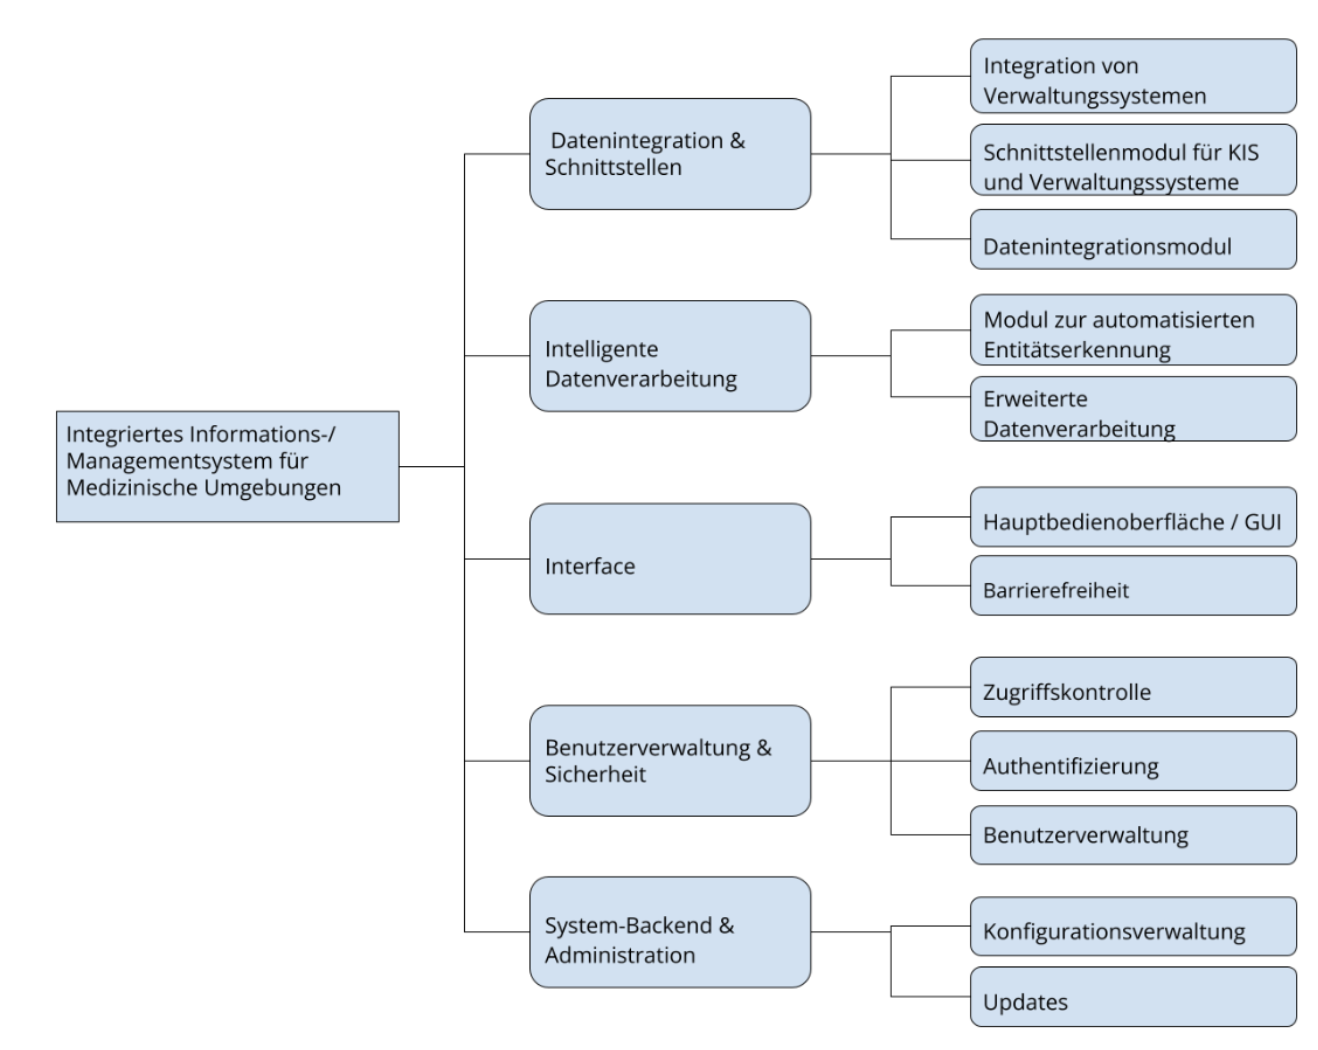
\includegraphics[width=1\textwidth]{fig/planung_alle_ebenen.png}
	\caption{Produktstrukturplan (PBS) des geplanten Systems}
	\label{fig:produktstrukturplan}
\end{figure}

Jede dieser Komponenten wurde weiter in Teilfunktionen und Module gegliedert, ohne zeitliche Abfolge, sondern mit dem Fokus auf die Zielstruktur des Endprodukts.

\subsection{Artefaktstrukturplan (ABS)}
\begin{figure}[ht]
	\centering
	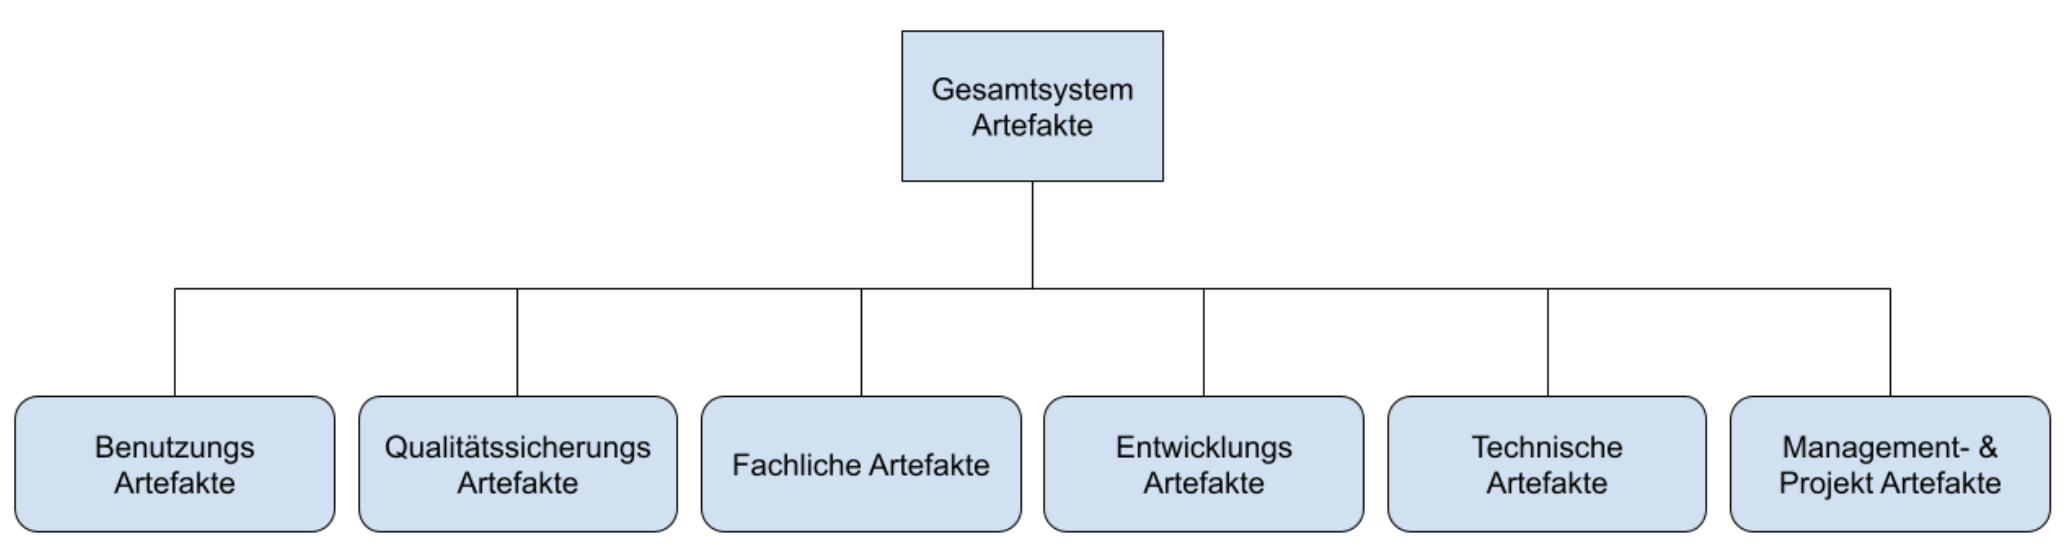
\includegraphics[width=1\textwidth]{fig/abs.png}
	\caption{Artefaktstrukturplan (ABS)}
	\label{fig:artefaktstrukturplan}
\end{figure}
Der Artefaktstrukturplan benennt die fachlichen, technischen, entwicklungsbezogenen, qualitativen und organisatorischen Artefakte, die im Entwicklungsverlauf entstehen. Dazu gehören unter anderem:

\begin{itemize}
	\item Anforderungsspezifikation, Stakeholderanalyse und Sicherheitsanforderungen
	\item Architekturdiagramme, Schnittstellenspezifikationen
	\item Annotierte Trainingsdaten, Code-Repositories, GUI-Prototypen
	\item Testkonzepte, Testergebnisse, Fehlermanagement
	\item Benutzer- und Administrationshandbücher
	\item Projektstrukturplan, Risikomatrix, Statusberichte
\end{itemize}

\subsection{Arbeitsstrukturplan (WBS)}
\begin{figure}[ht]
	\centering
	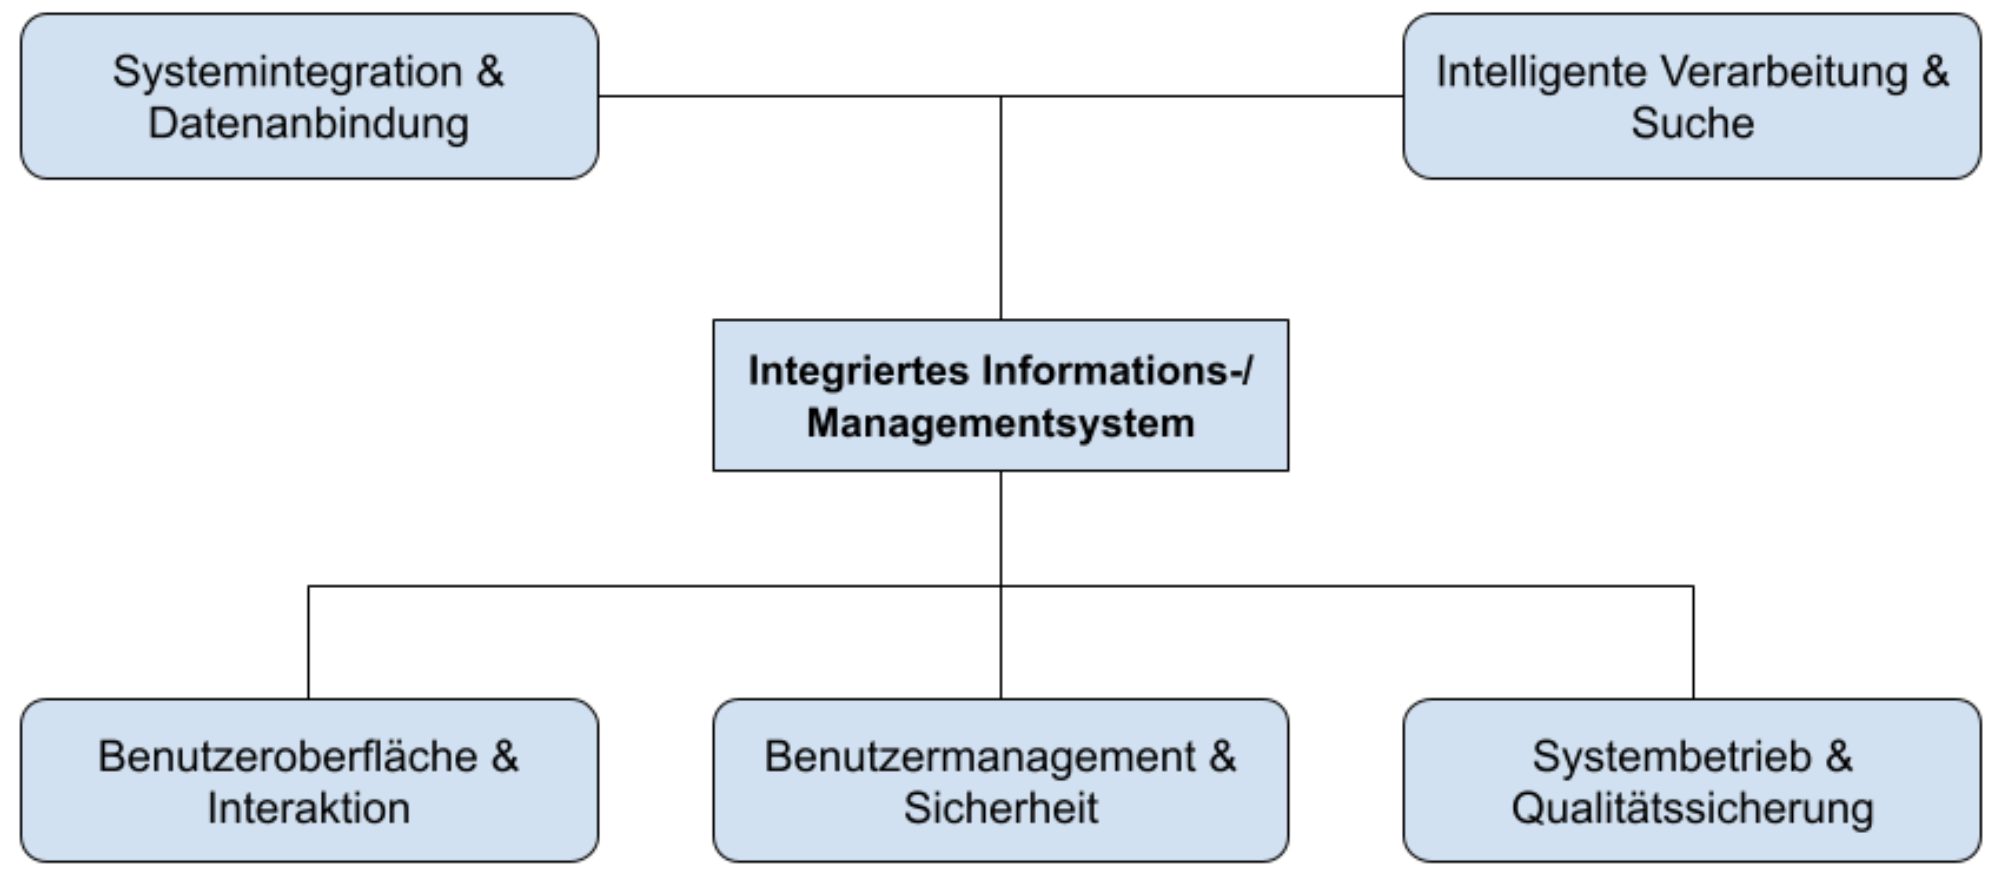
\includegraphics[width=1\textwidth]{fig/wbs.png}
	\caption{Arbeitsstrukturplan (WBS)}
	\label{fig:arbeitsstrukturplan}
\end{figure}
Der Arbeitsstrukturplan unterteilt das Projekt in konkrete Arbeitspakete (AP). Diese Pakete enthalten Angaben zu Inhalten, Zielen, Aufwand, Ressourcenbedarf und Abhängigkeiten. Beispiele sind:

\begin{itemize}
	\item \textbf{AP 1:} API-Integration für Verwaltungssysteme
	\item \textbf{AP 5:} Entwicklung eines NLP-Moduls zur medizinischen Entitätenerkennung
	\item \textbf{AP 9:} Authentifizierung und Zugriffskontrolle (inkl. SSO und 2FA)
\end{itemize}

Jedes Arbeitspaket wurde mit Leistungsfortschrittsindikatoren, geschätztem Aufwand in Personenstunden sowie Kosten versehen.
\pagebreak
\section{Konsistenzprüfung}
\begin{figure}[ht]
	\centering
	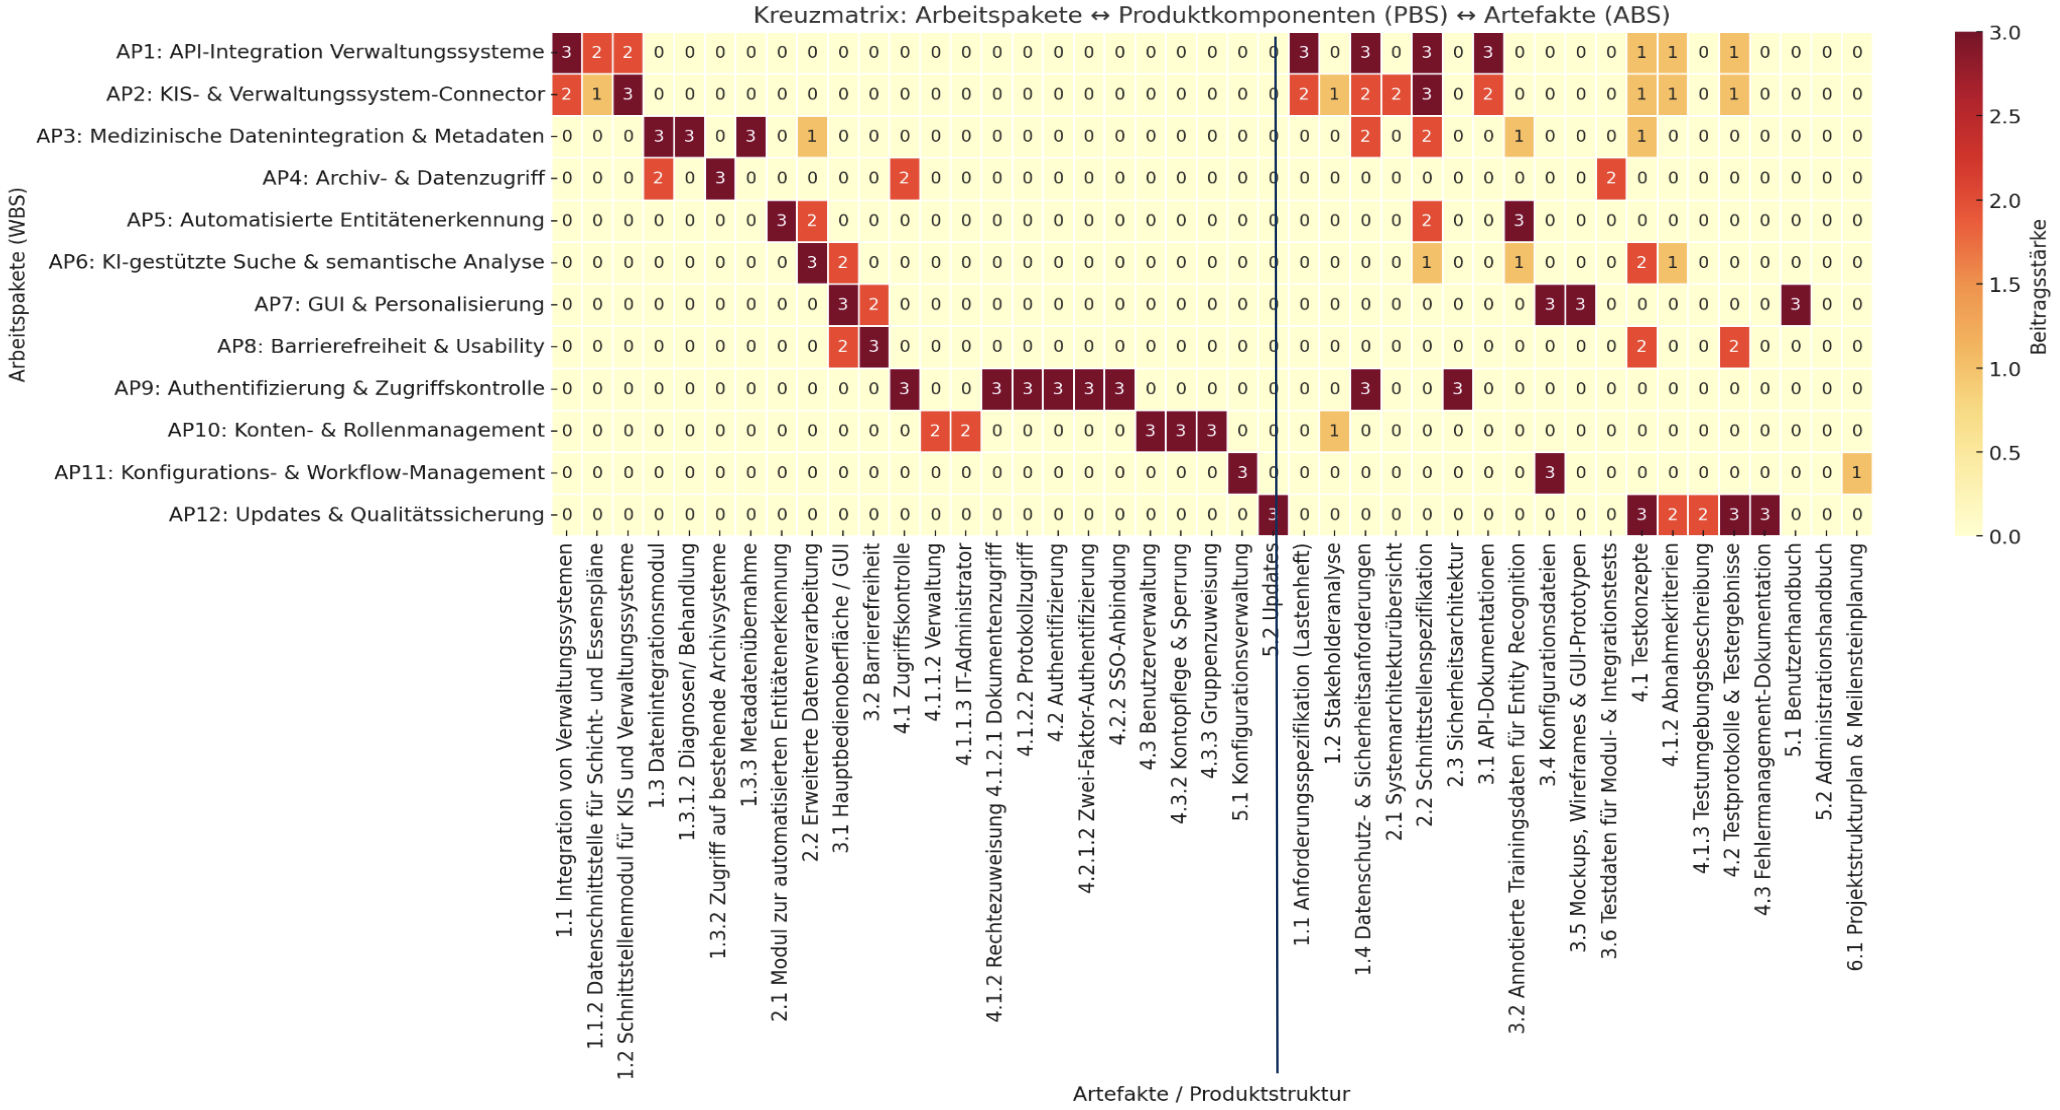
\includegraphics[width=1\textwidth]{fig/kreuzmatrix.png}
	\caption{Kreuzmatrix zur Konsistenzprüfung}
	\label{fig:kreuzmatrix}
\end{figure}
Im letzten Schritt wurde eine Kreuzmatrix verwendet, um die Konsistenz zwischen PBS, ABS und WBS zu prüfen. So konnten Lücken oder Inkonsistenzen frühzeitig identifiziert und behoben werden.

%\section{Fazit}
%Die durchgeführte Produktplanung bietet eine solide Basis für die weitere Projektumsetzung. Sie ermöglicht eine klare Ressourcenallokation, eine strukturierte Zeitplanung sowie die Definition von Teststrategien und Risikomanagementmaßnahmen. Besonders hervorgehoben wurden die Bereiche Datenintegration und Benutzerverwaltung, da sie zentrale Herausforderungen im Klinikalltag adressieren.

